\documentclass[pdftex,12pt,a4paper]{article}

\usepackage{graphicx}  
\usepackage[margin=2.5cm]{geometry}
\usepackage{breakcites}
\usepackage{indentfirst}
\usepackage{pgfgantt}
\usepackage{pdflscape}
\usepackage{float}
\usepackage{epsfig}
\usepackage{epstopdf}
\usepackage[cmex10]{amsmath}
\usepackage{stfloats}
\usepackage{multirow}
\renewcommand{\refname}{REFERENCES}
\linespread{1.3}
\usepackage{mathtools}
\graphicspath{{./images/}}

\usepackage{makecell}
\usepackage{nicematrix}
\usepackage{tabularx}
\usepackage{nicefrac}
\usepackage{nicematrix}
\usepackage{tikz}


%\newcommand{\HRule}{\rule{\linewidth}{0.5mm}}
\thispagestyle{empty}
\begin{document}
\begin{titlepage}
\begin{center}
\textbf{}\\
\textbf{\Large{ISTANBUL TECHNICAL UNIVERSITY}}\\
\vspace{0.5cm}
\textbf{\Large{COMPUTER ENGINEERING DEPARTMENT}}\\
\vspace{2cm}
\textbf{\Large{BLG 242E\\ DIGITAL CIRCUITS LABORATORY\\ EXPERIMENT REPORT}}\\
\vspace{2.8cm}
\begin{table}[ht]
\centering
\Large{
\begin{tabular}{lcl}
\textbf{EXPERIMENT NO}  & : & 1 \\
\textbf{EXPERIMENT DATE}  & : & 17.03.2023 \\
\textbf{LAB SESSION}  & : & FRIDAY - 16.00 \\
\textbf{GROUP NO}  & : & G18 \\
\end{tabular}}
\end{table}
\vspace{1cm}
\textbf{\Large{GROUP MEMBERS:}}\\
\begin{table}[ht]
\centering
\Large{
\begin{tabular}{rcl}
150220770  & : & ONUR BAYLAM \\
150200916  & : & DENIS IURIE DAVIDOGLU \\
\end{tabular}}
\end{table}
\vspace{2.8cm}
\textbf{\Large{SPRING 2023}}

\end{center}

\end{titlepage}

\thispagestyle{empty}
\addtocontents{toc}{\contentsline {section}{\numberline {}FRONT COVER}{}}
\addtocontents{toc}{\contentsline {section}{\numberline {}CONTENTS}{}}
\setcounter{tocdepth}{4}
\tableofcontents
\clearpage

\setcounter{page}{1}

\section{INTRODUCTION [10 points]}

Briefly describe what you have done during the experiment.

\section{MATERIALS AND METHODS [40 points]}
Answer all questions and provide everything that are indicated in the “Report” section of the related experiment in “Experiments Booklet”.
Edit following sub-heading as you wish.

\subsection{Preliminary}
\begin{figure}[H]
	\centering
	\includegraphics[width=0.5\textwidth]{logo.png}	
	\caption{An Example Figure Caption\cite{ref1}}
	\label{fig1}
\end{figure}

\subsection{Experiment}
\begin{itemize}
    \item \textbf{Part 1:} Design and implement the logic circuits for the given expressions below by using the necessary gates.\\
    $F_1 (a, b) = a + ab$ \\
    $F_2 (a, b) = (a + b) . (a + \overline{b})$\\

    \textbf{NOTE:} In order to design and implement boolean functions, we benefit from Logisim tool which enables us to simulate our circuits with different input combinations and detect possible errors.\\
    
    \newpage
    \textbf{Design of $F_1$:}\\
    To design and implement $F_1$, we need to use a 2-input AND gate, a 2-input OR gate.\\

    \begin{figure}[H]
    \centering
        \includegraphics[width=0.8\textwidth]{F1.png}	
        \caption{Design of \textbf{$F_1$} in Logisim}
   \end{figure}
   
   \begin{figure}[H]
    \centering
        \includegraphics[width=\textwidth]{EasyEDA_part_1_F1.png}	
        \caption{Design of \textbf{$F_1$} in EasyEDA}
   \end{figure}
   
   \textbf{Design of $F_2$:} \\ 
    To design and implement $F_2$, we need to use two 2-input OR gates, a 2-input AND gate, a NOT gate.\\

    \begin{figure}[H]
    \centering
        \includegraphics[width=0.8\textwidth]{F2.png}	
        \caption{Design of \textbf{$F_2$} in Logisim}
   \end{figure}

   \begin{figure}[H]
    \centering
        \includegraphics[width=\textwidth]{EasyEDA_part_1_F2.png}	
        \caption{Design of \textbf{$F_2$} in EasyEDA}
   \end{figure}
   
    \newpage
   To validate our designs of $F_1$ and $F_2$, we need to create truth tables of them. Both $F_1$ and $F_2$ functions have the same truth tables.\\
   \begin{figure}[H]
    \centering
        \includegraphics[width=0.25\textwidth]{f1truth.png}	
        \caption{Truth table of the function \textbf{$F_1$} and \textbf{$F_2$}}
   \end{figure}
   Our implementations of $F_1$ and $F_2$ are compatible with their truth table.\\
   
\end{itemize}
\begin{itemize}
    \item \textbf{Part 2:} A theorem is given as: $a + (a \cdot b) = a$. First, determine the dual of the given theorem and then, implement the functions for both sides of the dual theorem by using logic gates. Validate the truth of the theorem by comparing the changes in the outputs. \\
    
    First of all, the dual of a theorem is an expression created by replacing OR with AND, AND with OR, 1 with 0 and 0 with 1. Also, the order of operations should be preserved, so we need to put extra parentheses. In this formula, $(a \cdot b)$ is done first:
    
\begin{align*}
a + (a \cdot b) = a \tag{Original} \\
a \cdot (a+b) = a \tag{Dual} \\
\end{align*}

\begin{figure}[H]
\centering
\includegraphics[width=0.8\textwidth]{Logisim_part_2.png}	
\caption{Design in Logisim}
\end{figure}

\begin{figure}[H]
\centering
\includegraphics[width=\textwidth]{EasyEDA_part_2.png}	
\caption{Design in EasyEDA}
\end{figure}

To check validity of the dual theorem, the following truth table is constructed:

\begin{center}
\begin{tabular}{|c|c|c|c|c|c|}
\hline
$a$ & $b$ & $a \cdot b$ & $a+b$ & $a + a \cdot b$ & $a \cdot (a + b)$ \\
\hline
0 & 0 & 0 & 0 & 0 & 0 \\
0 & 1 & 0 & 1 & 0 & 0 \\
1 & 0 & 0 & 1 & 1 & 1 \\
1 & 1 & 1 & 1 & 1 & 1 \\
\hline
\end{tabular}
\end{center}
As it is clear from the table, the last two columns, which are the original expression's and its dual's left-hand side truth values, are identical to the first column, the right-hand side of the both equations. The equivalency of functions $a$ and $a \cdot (a+b)$ confirms the dual theorem. \\ 


\end{itemize}


\begin{itemize}
    \item \textbf{Part 3:} $F_3 (a, b, c) = ab + \overline{a}c$ is given. First, determine the complement of the given function ($F_3$). Then, implement the circuit which realizes the complementary function ($\overline{F_3}$). Validate your implementation by using the truth table.\\

    \textbf{Step 1:} In the first step, we find the complement of the given function $F_3$ by applying \textbf{De Morgan's} rule.\\
    
    Step 1.1: $\overline{F_3 (a, b, c)} = \overline{ab + \overline{a}c}$ \\
    
    Step 1.2: $\overline{F_3 (a, b, c)} = (\overline{a} + \overline{b}) . (a + \overline{c})$\\
    \newpage
    \textbf{Step 2:} In the second step, we implement the circuit which realizes the function $\overline{F_3}$.\\
    \begin{figure}[H]
    \centering
        \includegraphics[width=0.8\textwidth]{F3comp.png}	
        \caption{Design of \textbf{$\overline{F_3}$} in Logisim}
   \end{figure}
   
	\begin{figure}[H]
    \centering
        \includegraphics[width=\textwidth]{EasyEDA_part_3.png}	
        \caption{Design of \textbf{$\overline{F_3}$} in EasyEDA}        
	\end{figure}   
   
   \textbf{Step 3:} In the third step, we validate our implementation of the function $\overline{F_3}$ using truth table.\\
    \begin{figure}[H]
    \centering
        \includegraphics[width=0.3\textwidth]{truth.png}	
        \caption{Truth table of \textbf{$\overline{F_3}$}}
        \label{fig1}
   \end{figure}
    According to the truth table, our implementation is correct.
\end{itemize}

\begin{itemize}
    \item \textbf{Part 4:} A basic logical function $F_4$ is defined as follows.	
    $ F_4(a, b, c, d) = \cup_1 (1, 2, 5, 6, 9, 10, 13, 14) $.
    First, simplify given logical function and implement the simplified expression using logic gates. Validate your circuit by observing the outputs for each possible input. \\

Simplification is done using Karnaugh map. The result suggests only two prime implicants as show below:  

\begin{center}
  \begin{tabular}{c}
   \begin{tabular}{|c|c|}
  \hline
    ABCD & $F_4$ \\
    \hline
    0000 & 0 \\
    0001 & 1 \\
    0010 & 1 \\
    0011 & 0 \\
    0100 & 0 \\
    0101 & 1 \\
    0110 & 1 \\
    0111 & 0 \\
    1000 & 0 \\
    1001 & 1 \\
    1010 & 1 \\
    1011 & 0 \\
    1100 & 0 \\
    1101 & 1 \\
    1110 & 1 \\
    1111 & 0 \\
    \hline
  \end{tabular}
    
    $\quad$
    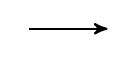
\begin{tikzpicture}[->,>=stealth', thick]
      \draw[->] (0,0) -- (1,0);
    \end{tikzpicture}
    $\quad$
    \begin{NiceTabular}{|w{l}{1cm}|c|c|c|c|}\hline
%\rule[-5mm]{5mm}{0cm}
\diagbox{AB}{CD}&
\Block{}{00}&\Block{}{01}&\Block{}{11}&\Block{}{10}\\
\hline
00 & 0 & 1 & 0 & 1\\
\hline
01 & 0 & 1 & 0 & 1\\
\hline
11 & 0 & 1 & 0 & 1\\
\hline
10 & 0 & 1 & 0 & 1\\
\hline
\end{NiceTabular}
    $\quad$
    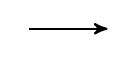
\begin{tikzpicture}[->,>=stealth', thick]
      \draw[->] (0,0) -- (1,0);
    \end{tikzpicture}
    $\quad$
    
     $ C\overline{D} + \overline{C}D $
  \end{tabular}
\end{center}

\begin{figure}[H]
    \centering
        \includegraphics[width=0.8\textwidth]{Logisim_part_4.png}	
        \caption{Design of \textbf{$F_4$} in Logisim}
   \end{figure}
   
	\begin{figure}[H]
    \centering
        \includegraphics[width=\textwidth]{EasyEDA_part_4.png}	
        \caption{Design of \textbf{$F_4$} in EasyEDA}        
	\end{figure}  

\end{itemize}
\begin{itemize}
    \item \textbf{Part 5:}
\end{itemize}

\begin{itemize}
    \item \textbf{Part 6:}
\end{itemize}
\section{RESULTS [15 points]}
Give the your results what did you get during the experiment. You can also add table, image, etc. 

\section{DISCUSSION [25 points]}
Please explain, analyze, and interpret what have you done during the  experiment. 

\section{CONCLUSION [10 points]}
Comment on any difficulties you have faced, what you have learned etc.

\newpage
\addcontentsline{toc}{section}{\numberline {}REFERENCES}

\bibliographystyle{unsrt}
\bibliography{reference}

\end{document}

